

\section{Aircraft Propeller}
An aircraft’s propeller consists of a rigid hub of radius $R$ and a flexible tapered blade of length $3R$ that has density $\rho (kg/m^3)$. The propeller is rotating about the center of the hub with a steady angular velocity $\omega$, thereby creating an effective axial distributed force in the blade. Neglect forces due to gravity. The cross sectional area distribution of the blade is $A(r)$, defined as

\begin{equation*}
    \input{q1/test}, \quad \text{if}\ R < r< 4R
\end{equation*}

\begin{figure}[h]
    \centering
    

\tikzset{every picture/.style={line width=0.75pt}} %set default line width to 0.75pt        

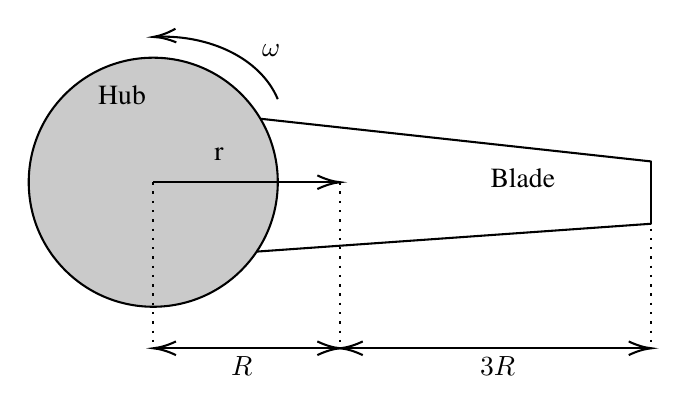
\begin{tikzpicture}[x=0.75pt,y=0.75pt,yscale=-1,xscale=1]
%uncomment if require: \path (0,300); %set diagram left start at 0, and has height of 300

%Shape: Circle [id:dp6244430308199536] 
\draw  [fill={rgb, 255:red, 202; green, 202; blue, 202 }  ,fill opacity=1 ] (220,120) .. controls (220,86.86) and (246.86,60) .. (280,60) .. controls (313.14,60) and (340,86.86) .. (340,120) .. controls (340,153.14) and (313.14,180) .. (280,180) .. controls (246.86,180) and (220,153.14) .. (220,120) -- cycle ;
%Straight Lines [id:da1433381310737285] 
\draw    (520,110) -- (520,140) ;
%Straight Lines [id:da6958270078143212] 
\draw    (520,110) -- (331.79,89.43) ;
%Straight Lines [id:da5982890152434965] 
\draw    (520,140) -- (329.79,153.43) ;
%Straight Lines [id:da7103183675633375] 
\draw    (280,120) -- (368,120) ;
\draw [shift={(370,120)}, rotate = 180] [color={rgb, 255:red, 0; green, 0; blue, 0 }  ][line width=0.75]    (10.93,-3.29) .. controls (6.95,-1.4) and (3.31,-0.3) .. (0,0) .. controls (3.31,0.3) and (6.95,1.4) .. (10.93,3.29)   ;
%Straight Lines [id:da18697245418380692] 
\draw  [dash pattern={on 0.84pt off 2.51pt}]  (280,120) -- (280,200) ;
%Straight Lines [id:da9445115873305969] 
\draw  [dash pattern={on 0.84pt off 2.51pt}]  (370,120) -- (370,200) ;
%Straight Lines [id:da8681269156370801] 
\draw    (282,200) -- (368,200) ;
\draw [shift={(370,200)}, rotate = 180] [color={rgb, 255:red, 0; green, 0; blue, 0 }  ][line width=0.75]    (10.93,-3.29) .. controls (6.95,-1.4) and (3.31,-0.3) .. (0,0) .. controls (3.31,0.3) and (6.95,1.4) .. (10.93,3.29)   ;
\draw [shift={(280,200)}, rotate = 0] [color={rgb, 255:red, 0; green, 0; blue, 0 }  ][line width=0.75]    (10.93,-3.29) .. controls (6.95,-1.4) and (3.31,-0.3) .. (0,0) .. controls (3.31,0.3) and (6.95,1.4) .. (10.93,3.29)   ;
%Straight Lines [id:da9459156094037822] 
\draw    (372,200) -- (518,200) ;
\draw [shift={(520,200)}, rotate = 180] [color={rgb, 255:red, 0; green, 0; blue, 0 }  ][line width=0.75]    (10.93,-3.29) .. controls (6.95,-1.4) and (3.31,-0.3) .. (0,0) .. controls (3.31,0.3) and (6.95,1.4) .. (10.93,3.29)   ;
\draw [shift={(370,200)}, rotate = 0] [color={rgb, 255:red, 0; green, 0; blue, 0 }  ][line width=0.75]    (10.93,-3.29) .. controls (6.95,-1.4) and (3.31,-0.3) .. (0,0) .. controls (3.31,0.3) and (6.95,1.4) .. (10.93,3.29)   ;
%Straight Lines [id:da5900923017563646] 
\draw  [dash pattern={on 0.84pt off 2.51pt}]  (520,120) -- (520,200) ;
%Curve Lines [id:da19047210809641868] 
\draw    (340,80) .. controls (331.57,59.94) and (306.65,48.98) .. (281.9,49.91) ;
\draw [shift={(280,50)}, rotate = 356.45] [color={rgb, 255:red, 0; green, 0; blue, 0 }  ][line width=0.75]    (10.93,-3.29) .. controls (6.95,-1.4) and (3.31,-0.3) .. (0,0) .. controls (3.31,0.3) and (6.95,1.4) .. (10.93,3.29)   ;

% Text Node
\draw (331,52.4) node [anchor=north west][inner sep=0.75pt]    {$\omega $};
% Text Node
\draw (316,202.4) node [anchor=north west][inner sep=0.75pt]    {$R$};
% Text Node
\draw (436,202.4) node [anchor=north west][inner sep=0.75pt]    {$3R$};
% Text Node
\draw (252,72) node [anchor=north west][inner sep=0.75pt]   [align=left] {{\fontfamily{ptm}\selectfont Hub}};
% Text Node
\draw (441,112) node [anchor=north west][inner sep=0.75pt]   [align=left] {{\fontfamily{ptm}\selectfont Blade}};
% Text Node
\draw (308,102) node [anchor=north west][inner sep=0.75pt]   [align=left] {{\fontfamily{ptm}\selectfont r}};


\end{tikzpicture}

\end{figure}
% Problem 1, a
%%%%%%%%%%%%%%%%%%%%%%%%%%%%%%%%%%%%%%%%%%%%%%%%%%%%%%%%%%%%%%%%%%%%%%%%%%%%%%%%%%%%%%%%%%%%%%%
\begin{enumerate}[label=\alph*., start = 1]
    \item Write down the expression for body force due to rotational acceleration. 
    
\end{enumerate}



\pagebreak
\pagestyle{fancy}
\restoregeometry



% Problem 1, b
%%%%%%%%%%%%%%%%%%%%%%%%%%%%%%%%%%%%%%%%%%%%%%%%%%%%%%%%%%%%%%%%%%%%%%%%%%%%%%%%%%%%%%%%%%%%%%%
\begin{enumerate}[label=\alph*., start = 2]
    \item In the 1D equilibrium equation derived in class, the area of cross section was constant. Show that the 1D equilibrium equation for the case of a changing cross sectional area is $\frac{d}{dr}(\sigma A) + fA = 0.$
\end{enumerate}

% Problem 1, c
%%%%%%%%%%%%%%%%%%%%%%%%%%%%%%%%%%%%%%%%%%%%%%%%%%%%%%%%%%%%%%%%%%%%%%%%%%%%%%%%%%%%%%%%%%%%%%%
\begin{enumerate}[label=\alph*., start = 3]
    \item  Write down the boundary conditions for the problem. 
\end{enumerate}

% Problem 1, d
%%%%%%%%%%%%%%%%%%%%%%%%%%%%%%%%%%%%%%%%%%%%%%%%%%%%%%%%%%%%%%%%%%%%%%%%%%%%%%%%%%%%%%%%%%%%%%%
\begin{enumerate}[label=\alph*., start = 4]
    \item Find the axial stress distribution, $\sigma(r)$
\end{enumerate}